\section{Direction of arrival using time delay information}
\subsection{Time delay between a single microphone pair}\label{sec:TDOA}

When using a pair of microphones, sound from a particular source arrives at the two microphones at different times, based on the source distance to the particular microphone. For a pair of microphones located at $m_{1}$ and $m_{2}$, the time difference of arrival (TDOA) of a sound signal from a source located at s can be defined as:
\begin{equation}
    \begin{split}
    T(\{m_{1},m_{2}\},s)&=\frac{|s-m_{1}|-|s-m_{2}|}{c}\\
                        &=\frac{|D_{1}|-|D_{2}|}{c}
    \label{eq:tdoa}
    \end{split}
\end{equation}
where c is the speed of sound in the medium and $|D_{1}|$ and $|D_{2}|$ the distance between the source and the microphones at $m_1$ and $m_2$.

In 2D, this equation leads to a hyperbola (Fig.\ref{eq:tdoa}) where the two focus points of the hyperbola are the sensors. The difference of the distance from any point of the hyperbola to the two focus is always the same.

\begin{figure}[H]
    \centering
    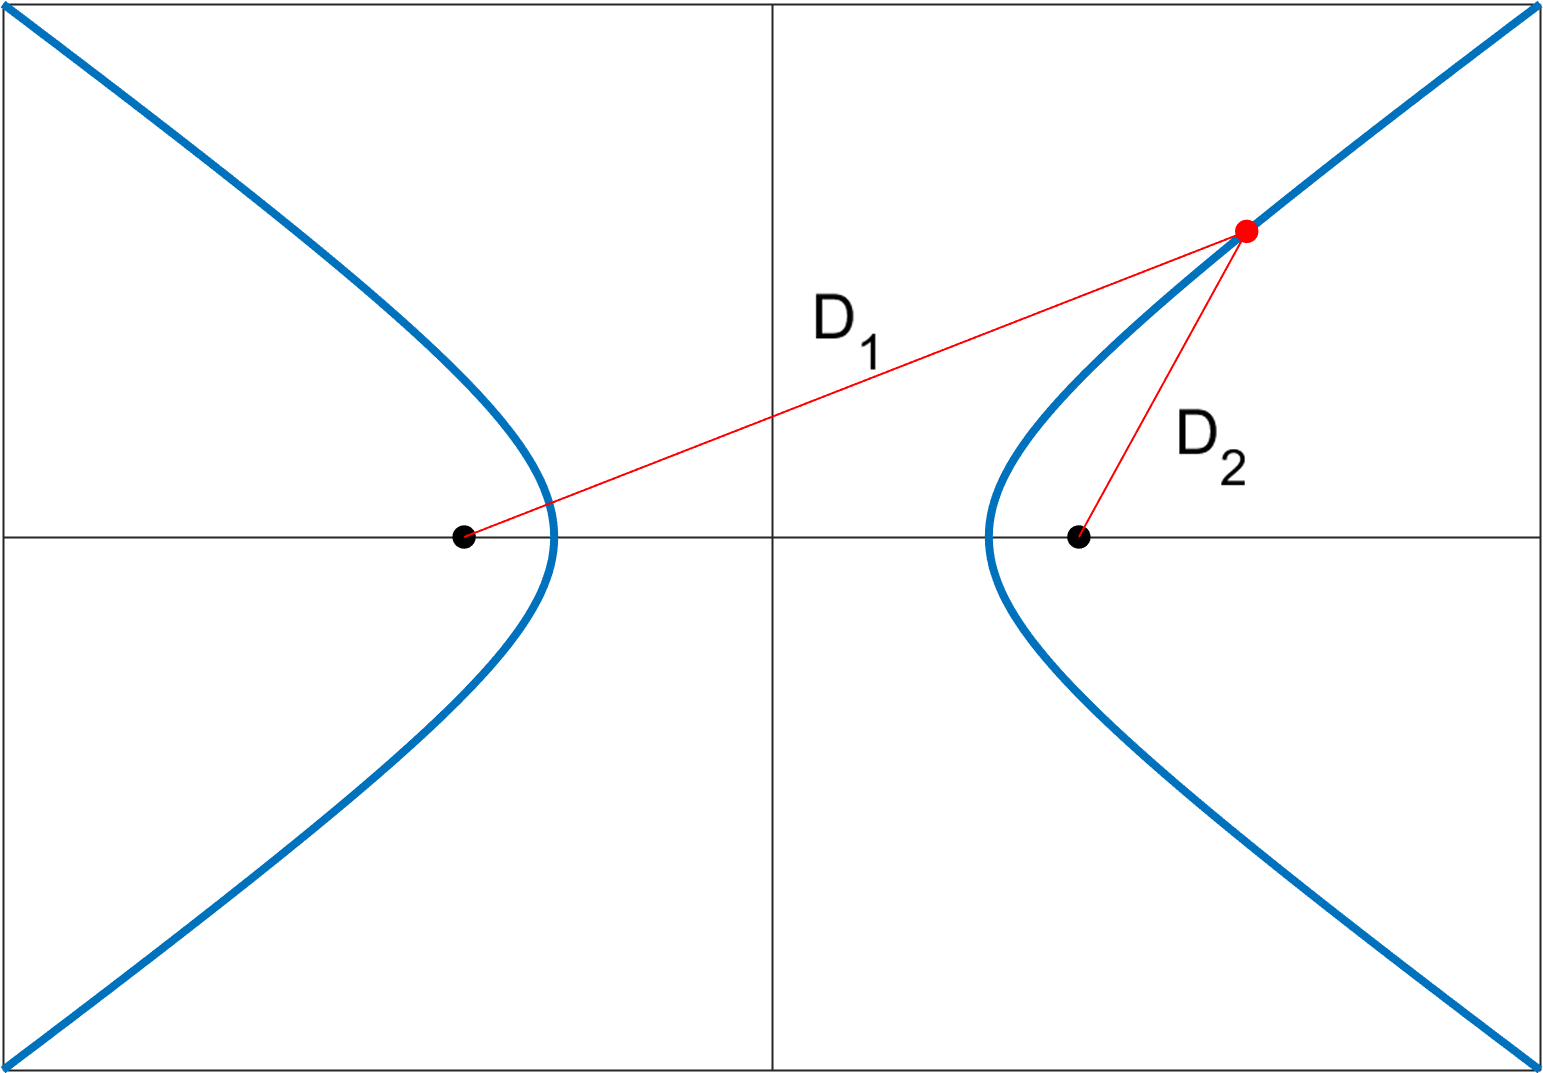
\includegraphics[width=0.8\textwidth]{Figures/hyperbola.png}
    \caption{A hyperbola (represented in blue), the red dot is any point on the hyperbola, the black dots represent the two foci. For any point on the hyperbola, $|D_1|-|D_2| = constant$}
    \label{eq:tdoa}
\end{figure}

In 3D, the TDOA information can be used to locate the source on a two-sheeted hyperboloid $\chi(\{m_{1},m_{2}\},s)$ such that the microphone positions are its foci. In practice the two-sheeted hyperboloid can be approximated to a cone so as to have a much simpler equation for the locus: $\theta$  = \textit{constant}, where $\theta$ is the angle of the source to the  midpoint of the line segment joining the two microphones (Fig. \ref{fig:hyperboloid_Cone}).

\begin{figure}[H]
    \centering
    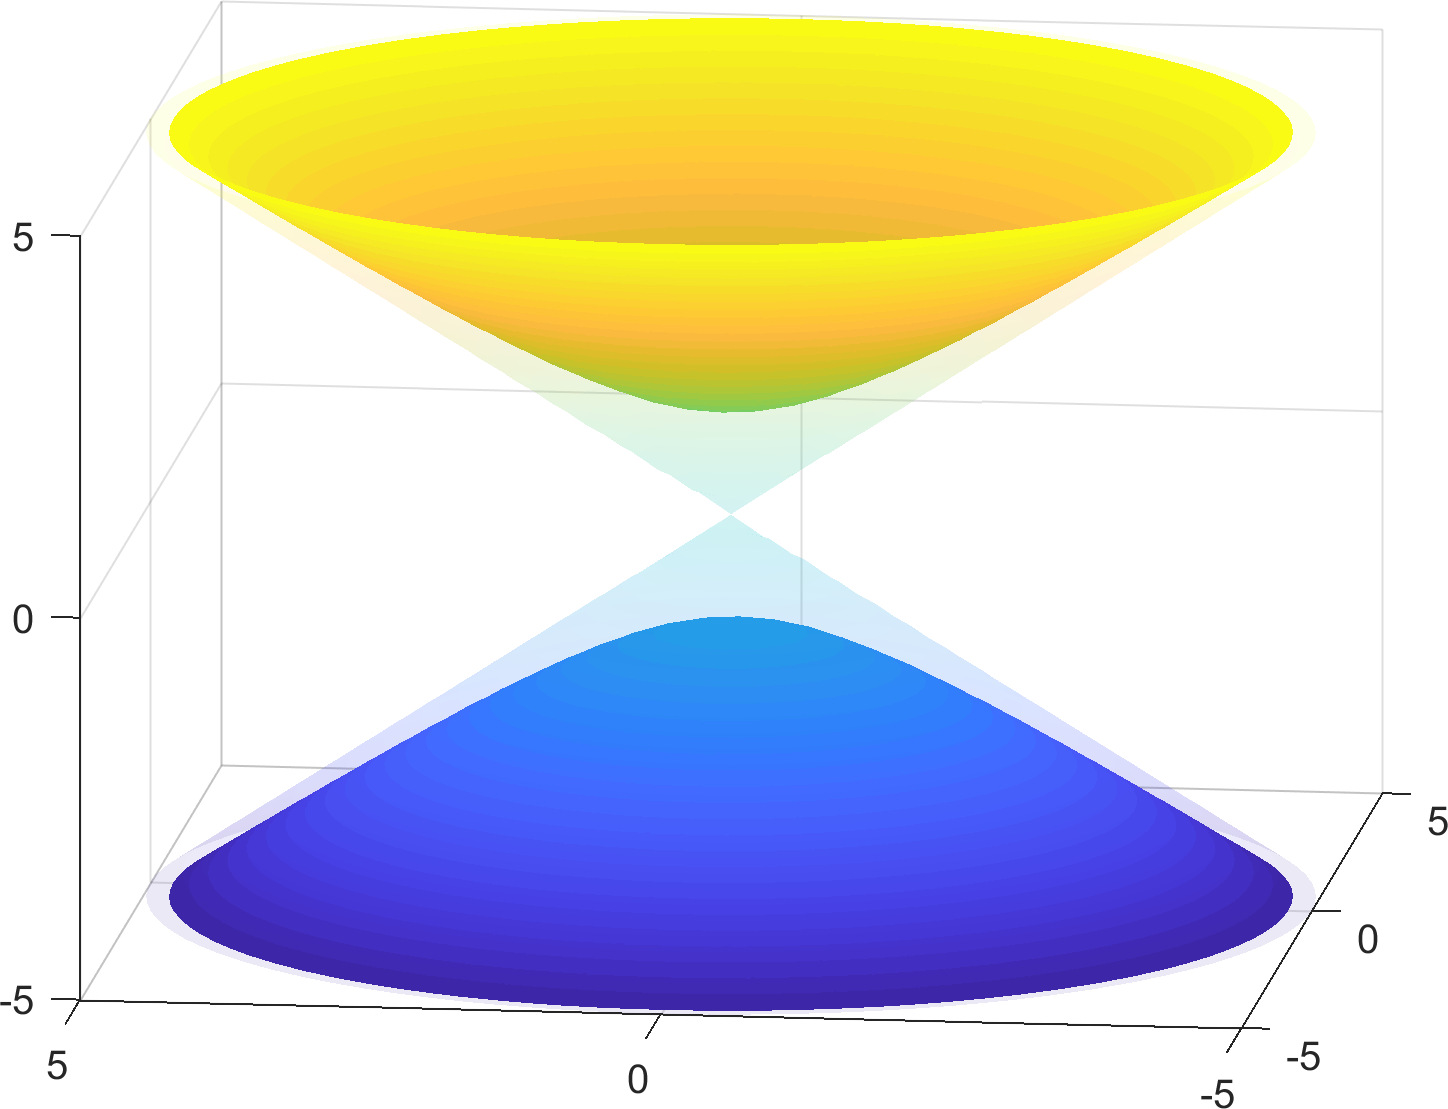
\includegraphics[width=0.8\textwidth]{Figures/hyperboloid.png}
    \caption{A 2-sheeted hyperboloid with a cone approximation overlay. As the tips of the hyperbola get closer (the microphones are closer), the hyperbola approximates the cone better.}
    \label{fig:hyperboloid_Cone}
\end{figure}

Of course as the source location gets closer to being orthogonal to the midpoint of the line segment joining the two microphones ($\theta=90\degree$), the hyperbola gets wider and flatter (more planar) and approximates the cone better. Also as the source gets closer to the line joining the two microphones ($\theta=0\degree, 180\degree$), the hyperbola collapses to a straight line and approximates the cone better. Thus, the error minimizes for broad-side sound source ($\theta=90\degree$) and for end-side sound source ($\theta=0\degree, 180\degree$), and maximizes for the midsection ($\theta=45\degree, 135\degree$). The equation for the error is given by
\begin{equation}
\begin{split}
    max\{\theta_{error}\} \approx  \frac{M_{dist}^2}{16R^2}\\
    max\{D_{error}\} \approx  \frac{M_{dist}^2}{16R},
\end{split}
\end{equation}
where $D_{error}$ is the actual source distance error (the gap between the cone and the hyperboloid) \cite{Brandstein:1995:FSS:922154}.

Microphones in microphone arrays are usually closely spaced with respect to the actual source distance, so the cone approximation works well. In most scenarios errors due to noise from other system parameters are greater than the errors associated with this approximation. Thus, given the time delay information between a microphone pair, the source can be located at a particular direction $\theta$, associated with the cone for that time delay, \textit{d}. 

It can be shown that the cone approximation is the same as a far-field assumption for the sound source. The far-field assumption leads to a planar wave-front for a uniform linear microphone array. Thus, for the far-field, the DOA estimation problem is essentially the same as the TDOA estimation problem as there is a one-to-one relation between $\theta$ and \textit{d}.

\begin{figure}
    \centering
    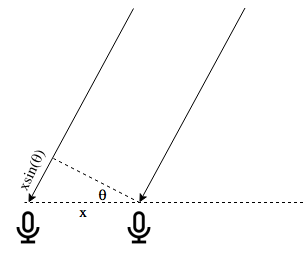
\includegraphics{Figures/Far-field.png}
    \caption{With far-field approximation it can be assumed that the sound waves incident on the pair of microphones are parallel (planar incidence).}
    \label{fig:my_label}
\end{figure}

Now, given the TDOA between multiple microphone pairs, the source localization problem can be solved by triangulation. This triangulation problem can be solved for different variables ($\theta$, Source Distance or the Time Delay itself). The next section will detail the basics of solving such a problem. 

\subsection{TDOA of N pair of microphones}\label{sec:TDOAN}

Each pair i of sensor gives a locus $\chi{i}(\{m_{i1},m_{i2}\},s)$ on which the source can be located. When more than one pair of sensor is used, the position of the source can be found at the intersection of each locus. Depending on the position of each sensor pair and the direction of arrival of the source, the intersection of all the locus could in theory be found $ ( s\in {\bigcap}_{i=0}^k \chi{i} )$. In practical, the DOA is corrupted by random noise process which influence the localization precision and therefore the locus of each microphone pair. In most case, the locus intersection is the empty set. $ ( {\bigcap}_{i=0}^k \chi{i} = \emptyset ) $


Figure \ref{fig:hyperboloid_intersect} gives a 2D representation of 3 hyperboloid intersecting. The problem is therefore how to estimate the best intersection and how does this estimation influence our TDOA. Solution to this problem are discussed in section \ref{sec:LSTDOA}

\begin{figure}[H]
    \centering
    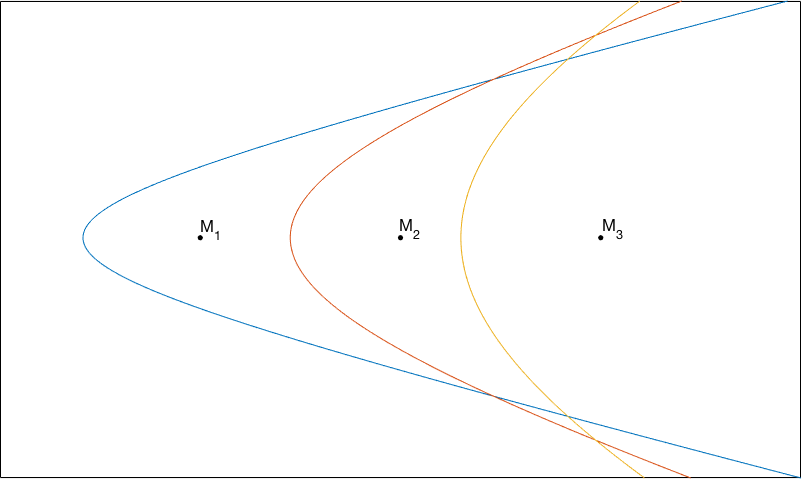
\includegraphics[width=0.8\textwidth]{Figures/intersect.png}
    \caption{2D representation of 3 locus. As seen above the intersection of the 3 locus is the empty set. $M_{1}$ , $M_{2}$ and $M_{3}$ represent the sensor position}
    \label{fig:hyperboloid_intersect}
\end{figure}

\subsection{Least Square problem}\label{sec:LSTDOA}

Let's define a Least Square (LS) problem which solves the localization of the sources in space as explained in section \ref{sec:TDOAN}. The LS problem optimize the position of the source in space by minimizing a given error criterion $ J $.
\begin{equation}
\hat{s}= \argmin_{s} J(s) 
\end{equation}

3 error criteria can be selected for solving the source location LS problem:  $J_{TDOA}(s)$, $J_{DOA}(s)$, $J_{D}(s)$. Those criteria are explained in the following sections.

\subsubsection{$J_{TDOA}(s)$ Error Criterion}

$J_{TDOA}(s)$ is the squared error difference between the time delay estimate $\tau$ and the time delay measured between the microphone pairs. The criterion and the optimization problem is given in the following.

\begin{equation}
J_{TDOA}(s) = {\sum}_{i=0}^k \epsilon_{itdoa}.[\tau_{i}-T(\{m_{i1},m_{i2}\},s)]^2
\label{eq:jtdoa}
\end{equation}
\begin{equation}
\hat{s}_{tdoa}= \argmin_{s} J_{tdoa}(s) 
\end{equation}

Assuming that the TDOA estimates $\tau_{i}$ are independently corrupted by zero-mean white gaussian noise, the stochastic variable $\mathcal{T}_{i}$ associated with this random process follows a normal distribution. The likelihood function of such a distribution is well-known and therefore the log of the distribution likelihood can be maximized yielding the Maximum Likelihood (ML) estimate of the TDOA from which the estimated position can be computed . 

Note that the error criterion is scaled by a factor $\epsilon_{itdoa}$ which is the inverse of the TDOA estimate $\mathcal{T}_{i}$ variance. 

\begin{equation}
\epsilon_{itdoa}=\frac{1}{\mathrm{Var}{\mathcal{T}_{i}}}
\label{eq:epsilonjtdoa}
\end{equation}

\subsubsection{$J_{DOA}(s)$ Error Criterion}

This is a classical formulation of the problem, which follows the same idea as the TDOA error criterion but this time the $J_{DOA}(s)$ is the squared error difference between the DOA estimate $\theta$ and the DOA measured between the microphone pairs. 

\begin{equation}
J_{DOA}(s) = {\sum}_{i=0}^k \epsilon_{idoa}.[\Theta_{i}-\theta(\{m_{i1},m_{i2}\},s)]^2
\label{eq:jdoa}
\end{equation}
\begin{equation}
\hat{s}_{doa}= \argmin_{s} J_{doa}(s) 
\end{equation}


Assuming that the DOA estimates $\theta_{i}$ are independently corrupted by zero-mean additive white Gaussian noise, the stochastic variable $\Theta_{i}$ associated with this random process follow a normal distribution. The error criterion is also scaled by a factor $\epsilon_{idoa}$ which is the inverse of the DOA estimate $\Theta_{i}$ variance. 

\begin{equation}
\epsilon_{idoa}=\frac{1}{\mathrm{Var}{\Theta_{i}}}
\label{eq:epsilonjtdoa}
\end{equation}

\subsubsection{$J_{D}(s)$ Error Criterion}

finally, $J_{D}(s)$ is the squared error difference between the orthogonal distance from s to the appropriate cone approximation 

\begin{equation}
J_{DOA}(s) = {\sum}_{i=0}^k \epsilon_{id}.[D(\chi_{i},s)]^2
\label{eq:jd}
\end{equation}
\begin{equation}
\hat{s}_{d}= \argmin_{s} J_{d}(s) 
\end{equation}


\begin{equation}
D(\chi_{i},s)=R_{i}.\sin{[\theta_{i}-\Theta(m_{i1},m_{i2},s)}]  
\end{equation}

\begin{equation}
 \epsilon_{id}=\frac{1}{\mathrm{Var}{\Theta_{i}}}    
\end{equation}

\subsubsection{Estimator performance}

The estimators described above vary in term of performance under certain conditions. For a bi-linear array, Brandstein has shown that $J_{TDOA}(s)$ and $J_{DOA}(s)$ are more robust to great angle of incidence than $J_{D}(s)$. At low noise level, $J_{TDOA}(s)$ is proven to be slightly better than $J_{DOA}(s)$ but $J_{DOA}(s)$ perform better overall especially for long range source location. $J_{TDOA}(s)$ is better for broadside sources and low noise level but $J_{DOA}(s)$ is more robust for less favorable noise conditions

%Pros and Cons of each estimators are sumarized in the following table.